\documentclass[a4paper,UKenglish,cleveref,thm-restate]{lipics-v2021}
\nolinenumbers

\title{Range Minimum Queries}
\author{Emirhan Yilmaz}{Karlsruhe Institute of Technology, Germany}{}{}{}
\hideLIPIcs

\begin{document}
\maketitle


\section{Introduction}
This project is my submission for the programming Project for the Advanced Data Structures course, Summer 2026.
This project was implemented in C++, where the source file can be found under the directory $\texttt{rmq-cpp}$.

\section{Methods}
\subsection{Naive}
The naive implementation is the most uninteresting; for queries, the algorithm iterates over each individual value in the range. 
- Runtime Complexity: $\mathcal{O}(n)$
	- As we calculate the minimum for a given range naively, this approach is the slowest among all the implemented algorithms
- Space Complexity: $\mathcal{O}(1)$
	- The only rather positive property of this algorithm is that it uses the least amount of additional space among all other algorithms, which is just a pointer to the original data and nothing more
\subsection{Precompute everything}
This approach lies on the other end of the time/space tradeoff spectrum as the naive implementation. Here, every possible query is precomputed and stored in a table -- evey range minimum query corresponds to a lookup in this table. The table is a vector of size $\frac{n^2}{2} + \frac{n}{2}$ and correspond to the upper triangular part of an $n \times n$ matrix. 
- Runtime Complexity: $\mathcal{O}(1)$
	- Each query $\[l, r\]$ is stored at index $ln -  \frac{l(l - 1)}{2} + (r - l)$, which must be calculated for every query. A query then corresponds to a simple lookup in the aforementioned table.
- Space Complexity: $\mathcal{O}(n^2)$
\subsection{Sparse Arrays}
Instead of calculating every single answer for a query, we can instead precalculate every range whose length is a power of two while still having constant-time lookups and eliminating the massively impractical quadratic runtime of precalculating every answer. This approach utilizes nested vectors, with the inner vectors storing the minimum of ranges with the length of powers of 2 and the outer vector storing these levels. Querying this array consists of first computing the level which we need to compare the minimums of, accessing the two values in our table and then taking the minimum, which allows for querying in $\mathcal{O}(1)$.
- Runtime Complexity: $\mathcal{O}(1)$
- Space Complexity: $\mathcal{O}(n log n)$
	- There are $log n$ levels with each level having $n - 2^k + 1$ intervals. 
\subsection{Segment Trees}
Many of the intervals computed in sparse arrays overlap and we can omit this redundancy at the cost of querying time. we again have nested nested vectors where the outer vector represents levels and the inner vectors represent the minima of segments in the respective level.  
- Runtime Complexity: $\mathcal{O}(log n)$
	- The algorithm recursively checks whether the left or right boundary already aligns with a complete segment by descending through the tree.
- Space Complexity: $\mathcal{O}(n)$
	- There are $log n$ levels with each level having at most half the number entries from the previous level resulting in at most $2n$ needed additional space.
\subsection{Blocks}
Here, the idea is to split the input into blocks of a fixed size and precompute the minimum of each block. I have implemented three types of block-based range minimum querying. One, where the suffix and prefix minima of the start and end blocks respectively are calculated on the fly, another one where these prefixes and suffixes are precomputed for each block, and another one where each combination of the middle blocks are precalculated as well.
\subsubsection{On-The-Fly Pre-/Suffixes}
Since the prefixes and suffixes are calculated on the fly, we only need one additional vector for the blocks. During building, we simply iterate through all values in every block and assign it its minimum value. 
- Runtime Complexity: $\mathcal{O}(\sqrt{n})$

- Space Complexity: $\mathcal{O}(n)$

\subsubsection{Precalculating Pre-/Suffixes}
In this, we have two additional vectors of size $n$ one populated with the minimum of the entries to the start of the next block and another from the end of the previous block to the current entry.
- Runtime Complexity: $\mathcal{O}(\sqrt{n})$
- Space Complexity: $\mathcal{O}(n)$
\subsubsection{Precalculating Block Queries}
It is possible to even bring down the query time to constant time by precalculating the queries on the middle blocks similar to the previous sparse array algorithm. Each query therefore now only comprises a lookup in prefix array, suffix array, and the sparse table for the blocks.
- Runtime Complexity: $\mathcal{O}(1)$
- Space Complexity: $\mathcal{O}(n log n)$
\subsection{Cartesian Trees}
Like in the block based approach, this algorithm divides the input data into small blocks. The main difference is that it exploits the fact that many blocks have the same relative structure, allowing the algorithm to reuse precomputed lookup tables instead of building one for every block. If the query is completely within a single block, we find the corresponding block shape, look up the index of the minimum inside that range, and return the orignal value. If the query spans multiple block, the query is divided into a left partial block lookup, a right partial block lookup and a lookup of the minimum over the queried blocks in a lookup table.  
- Runtime Complexity: $\mathcal{O}(1)$
At most two lookup table accesses and one sparse table query are performed.
- Space Complexity: $\mathcal{O}(n)$
Only one lookup table is stored per distinct block shape. By choosing a block size of roughly $\frac{1}{4} log_2 n$, the number and size of all possible shape tables together remain linear in n.
\section{Results}
\begin{figure}[h]
	\centering
	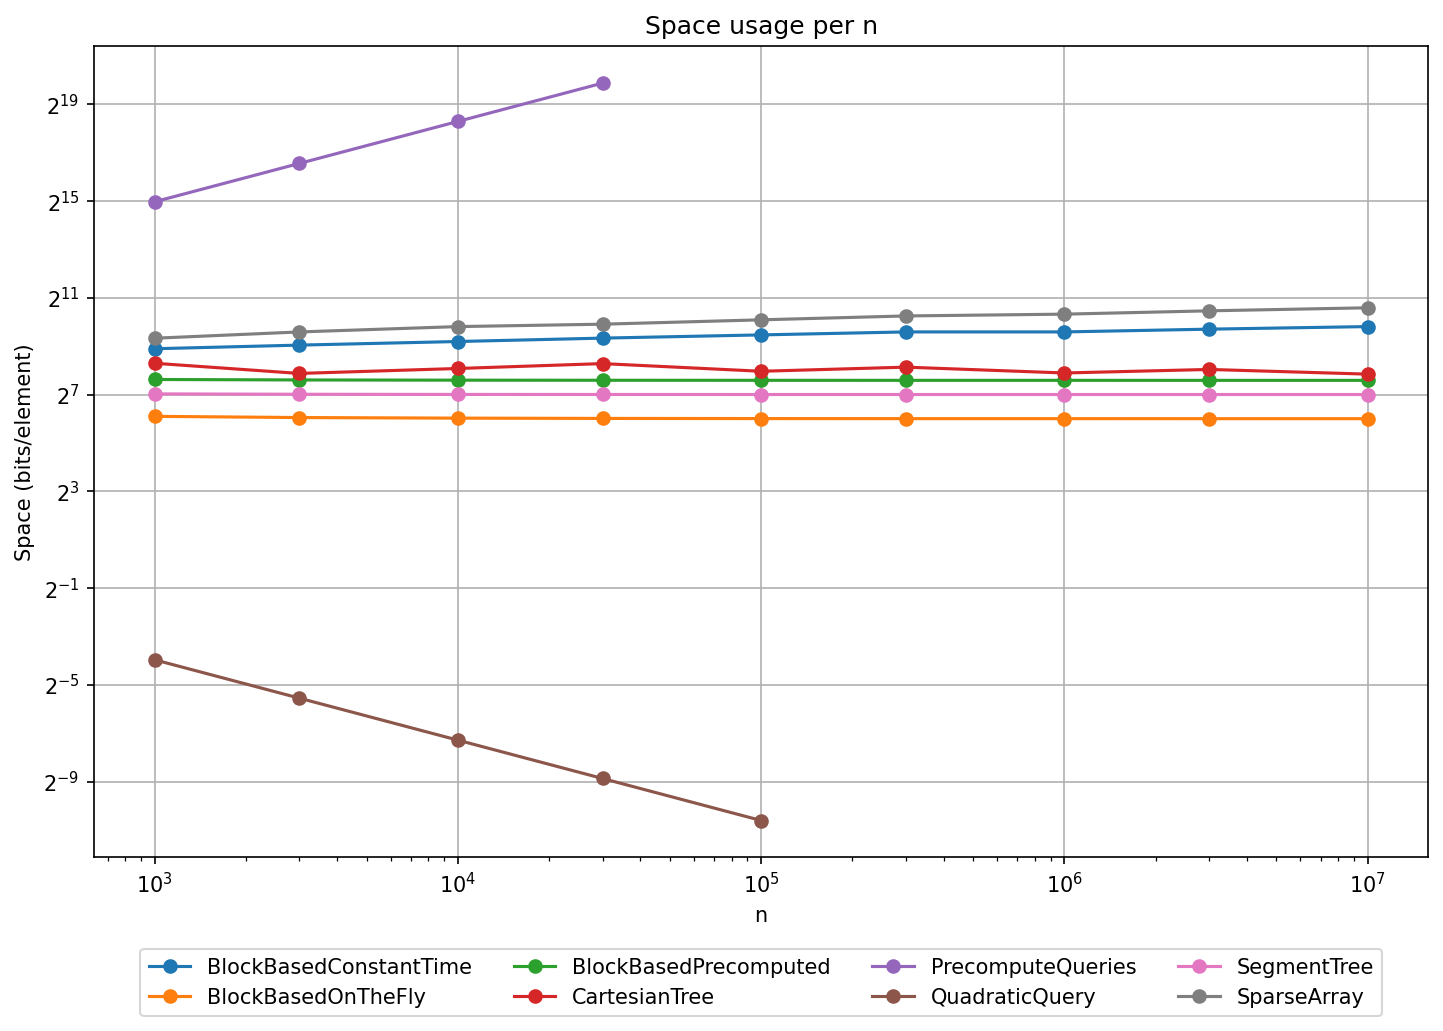
\includegraphics[width=.8\linewidth]{../plots/space.png}
	\caption{space usage}
\end{figure}
\begin{figure}[h]
	\centering
	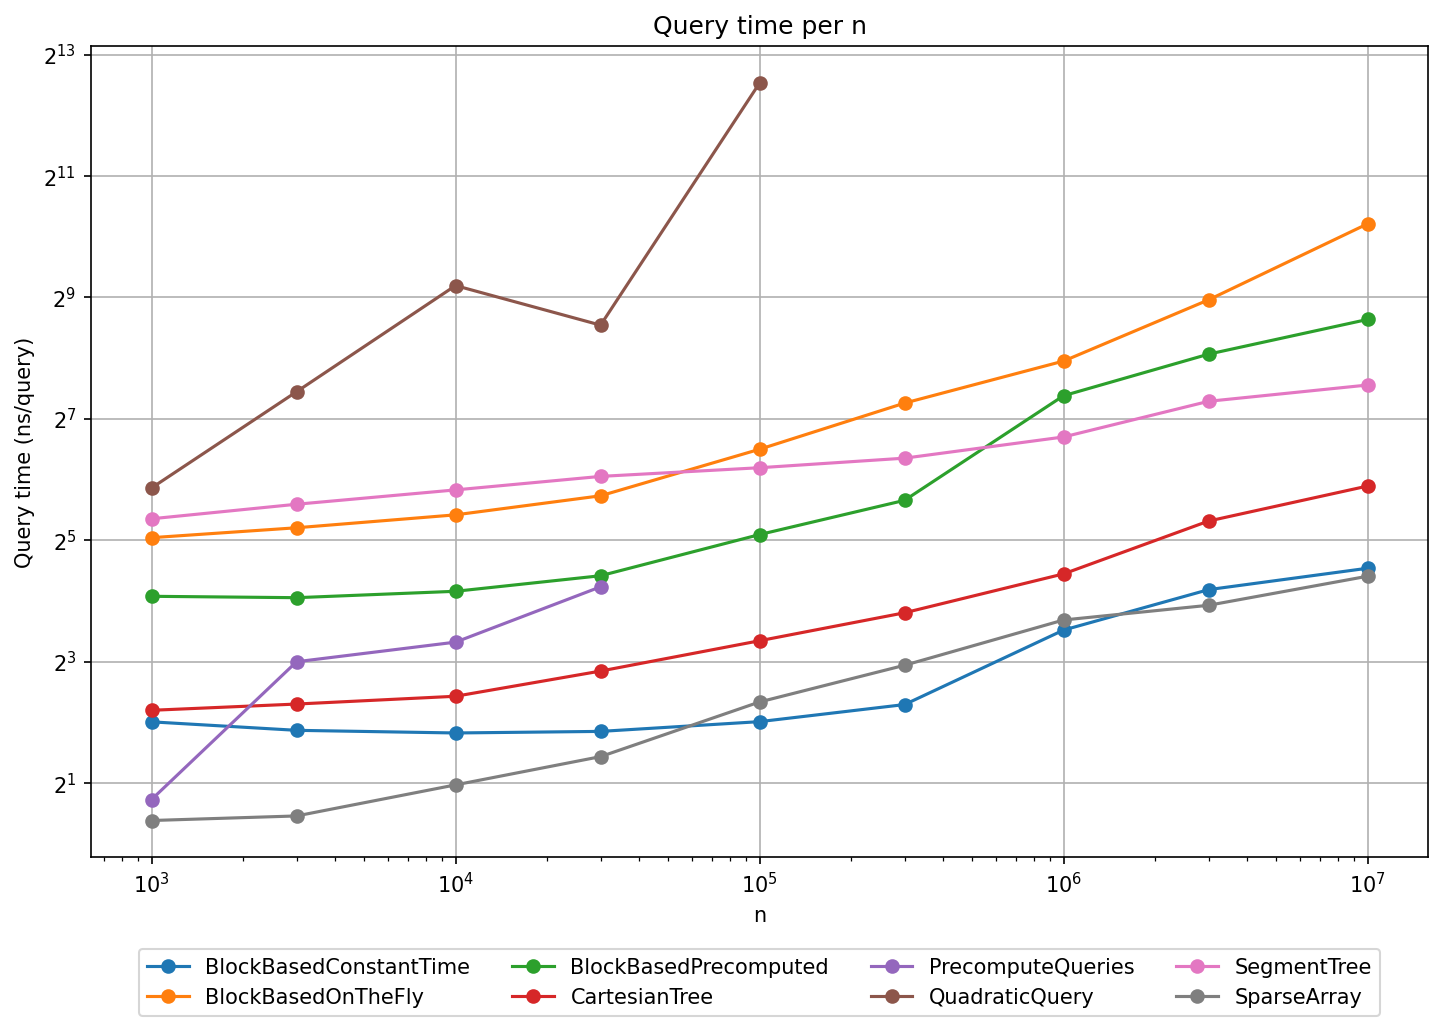
\includegraphics[width=.8\linewidth]{../plots/query_time.png}
	\caption{query time}
\end{figure}
\begin{figure}[h]
	\centering
	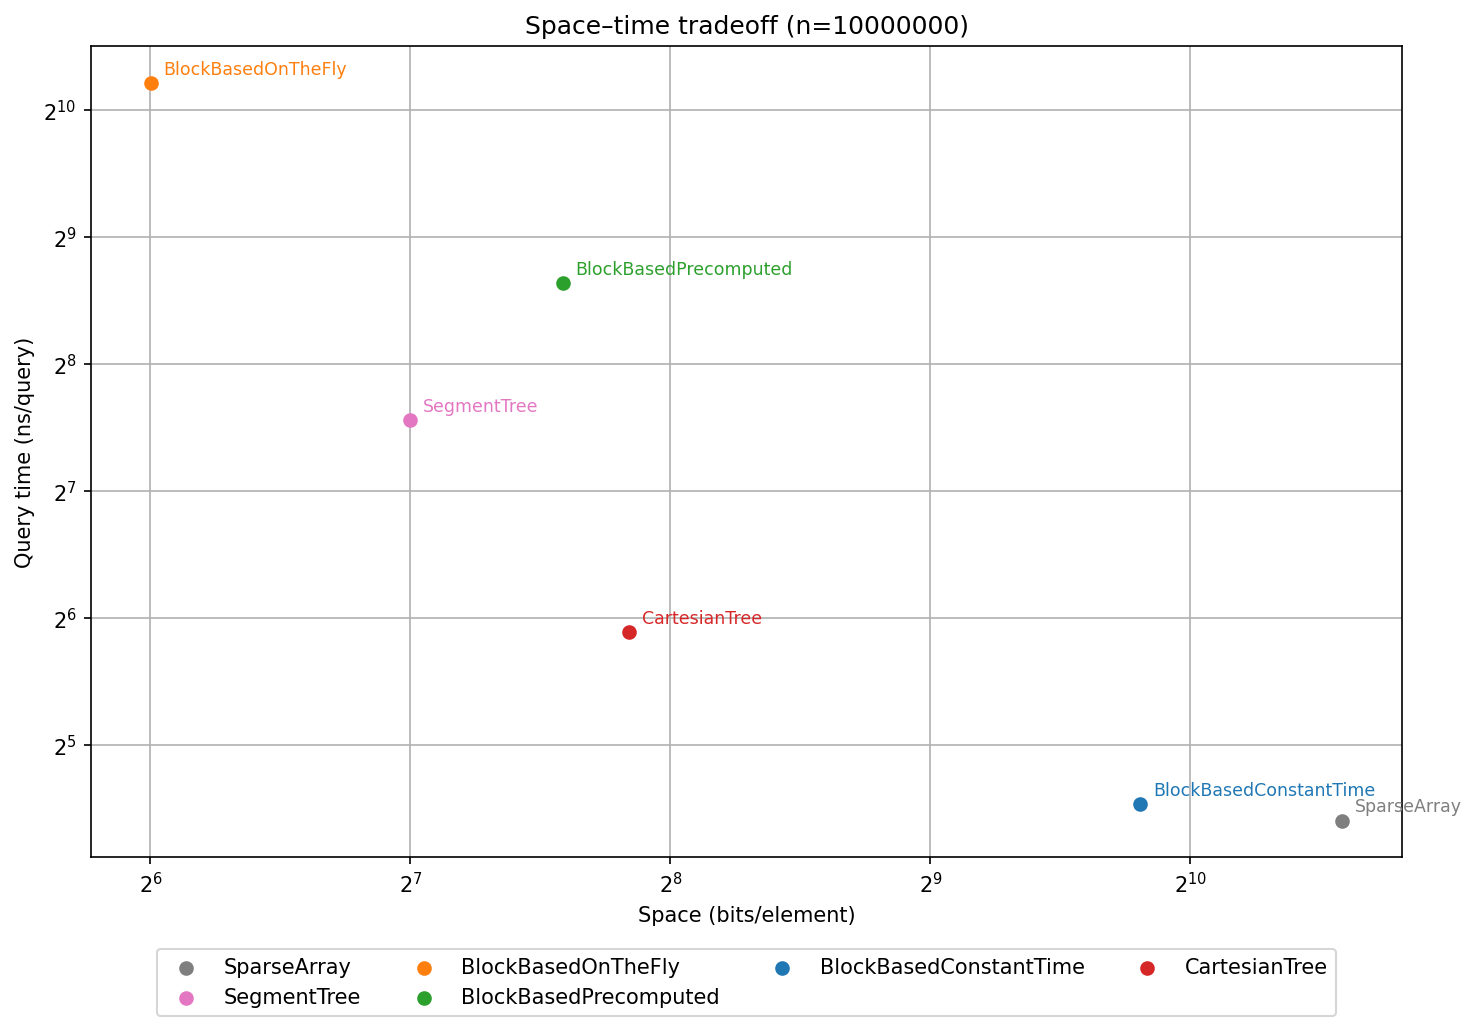
\includegraphics[width=.8\linewidth]{../plots/space_time_tradeoff.png}
	\caption{space-time trade-off}
\end{figure}

\subsection{Space Usage}
Overall, the measured memory consumption closely matches the theoretical expectations.

As expected, precomputing every possible query consumes the largest amount of memory and becomes very impractical for larger $n$.

Looking at the plot for the space usage, it can be seen that the block based constant-time approach and the sparse array algorithms require more memory per $n$ for larger $n$ matches the theoretical $\mathcal{O}(n log n)$ while Segment Tree, Cartesian Tree and the other block-based approaches similarly match their theoretical space requirement $\mathcal{O}(n)$ 
\subsection{Query Times}
The benchmark results of the constant-time algorithms does not exactly align with the expected query timings. As $n$ increases, the time per query for these algorithms also slightly increases, despite the constant asymptotic runtime. However, this observation does not necessarily contradict the measured runtime. 

Lookups and queries to the internal data structures of these algorithms are heavily affected by cache related latencies. For example, for small $n$, the used data structures neatly fit into the CPU cache, whereas this can no longer be the case for larger $n$, resulting in more cache misses leading to worse querying performance.  

The benchmark results of the other algorithms coarsely follow the expected asymptotic runtime. As can be seen in the chart, the segment tree algorithm  with an asymptotic runtime of $\mathcal{O}(n log)$ catches up with the $\mathcal{O}(\sqrt{n})$ runtime of the on-the-fly and precomputed variants of the block-based approaches.
\subsection{Pareto-Optimalness}
Not considering on-the-fly querying and precomputing queries for practicality reasons, the on-the-fly block-based approach is by far the most space efficient algorithm while the algorithm using the sparse array has the fastest practical queries as it is algorithm with the smallest cache footprint. 
Considering both memory usage and query time, the cartesian tree shows a favorable trade-off between those two. It for $n = 10.000.000$, it requires $\times 6,7$ less memory than the fastest algorithm while only being $\times 2,3$ slower.
\subsection{Parameters}
Among the compared algorithms, only the block-based approaches require selecting an appropriate block-size.
While small blocks increase the total number of blocks, making the sparse table larger, bigger blocks decrease the total number of blocks but making intra-block querying require more work.
Choosing a block size of $\[
s = \max\left(1,\; 2^{\left\lfloor \frac{\log_2 n}{2} \right\rfloor}\right)
\]$ yields good querying performance while also keeping the memory footprint reasonable.
\end{document}